\documentclass[11pt]{article}
\usepackage[margin=1in]{geometry}
\usepackage{booktabs}
\usepackage{graphicx}
\usepackage{microtype}
\usepackage[hidelinks]{hyperref}

\newcommand{\rzFrontier}{5.15}
\newcommand{\reFrontier}{30.81}


\title{\vspace{-2em}\textbf{Recency knob --- a control surface, not a winner}}
\author{arxivkg · generation · recency knob}
\date{}

\begin{document}
\maketitle
\vspace{-2em}

\section*{What we did}
Sweep the topic-adaptive recency knob \texttt{recency} $\in \{0.0, 0.2, 0.4, 0.6, 0.8\}$ over the
27-topic battery. The knob dials how many landmark slots are reserved newest-cohort-first (frontier)
versus left to PPR lineage ranking; the frontier \emph{year} is auto-detected per topic from its own
histogram, so the knob is a relative dial, not an absolute year.

\section*{Results (mean over 27 topics)}
\begin{center}\begin{tabular}{lrrrrrrr}
\toprule
recency & frontier count & ge 2025 & n 2026 & n edges & grounded & off digest & landmark recall \\
\midrule
0.0 & 5.15 & 1.26 & 0.78 & 4994.04 & 21.11 & 0.19 & 0.09 \\
0.2 & 10.56 & 4.0 & 1.56 & 4994.04 & 22.07 & 0.22 & 0.09 \\
0.4 & 16.78 & 7.0 & 2.07 & 4994.04 & 23.74 & 0.04 & 0.09 \\
0.6 & 23.56 & 9.7 & 2.26 & 4994.04 & 23.85 & 0.26 & 0.05 \\
0.8 & 30.81 & 12.59 & 2.44 & 4994.04 & 22.37 & 0.07 & 0.04 \\
\bottomrule
\end{tabular}
\end{center}
\begin{center}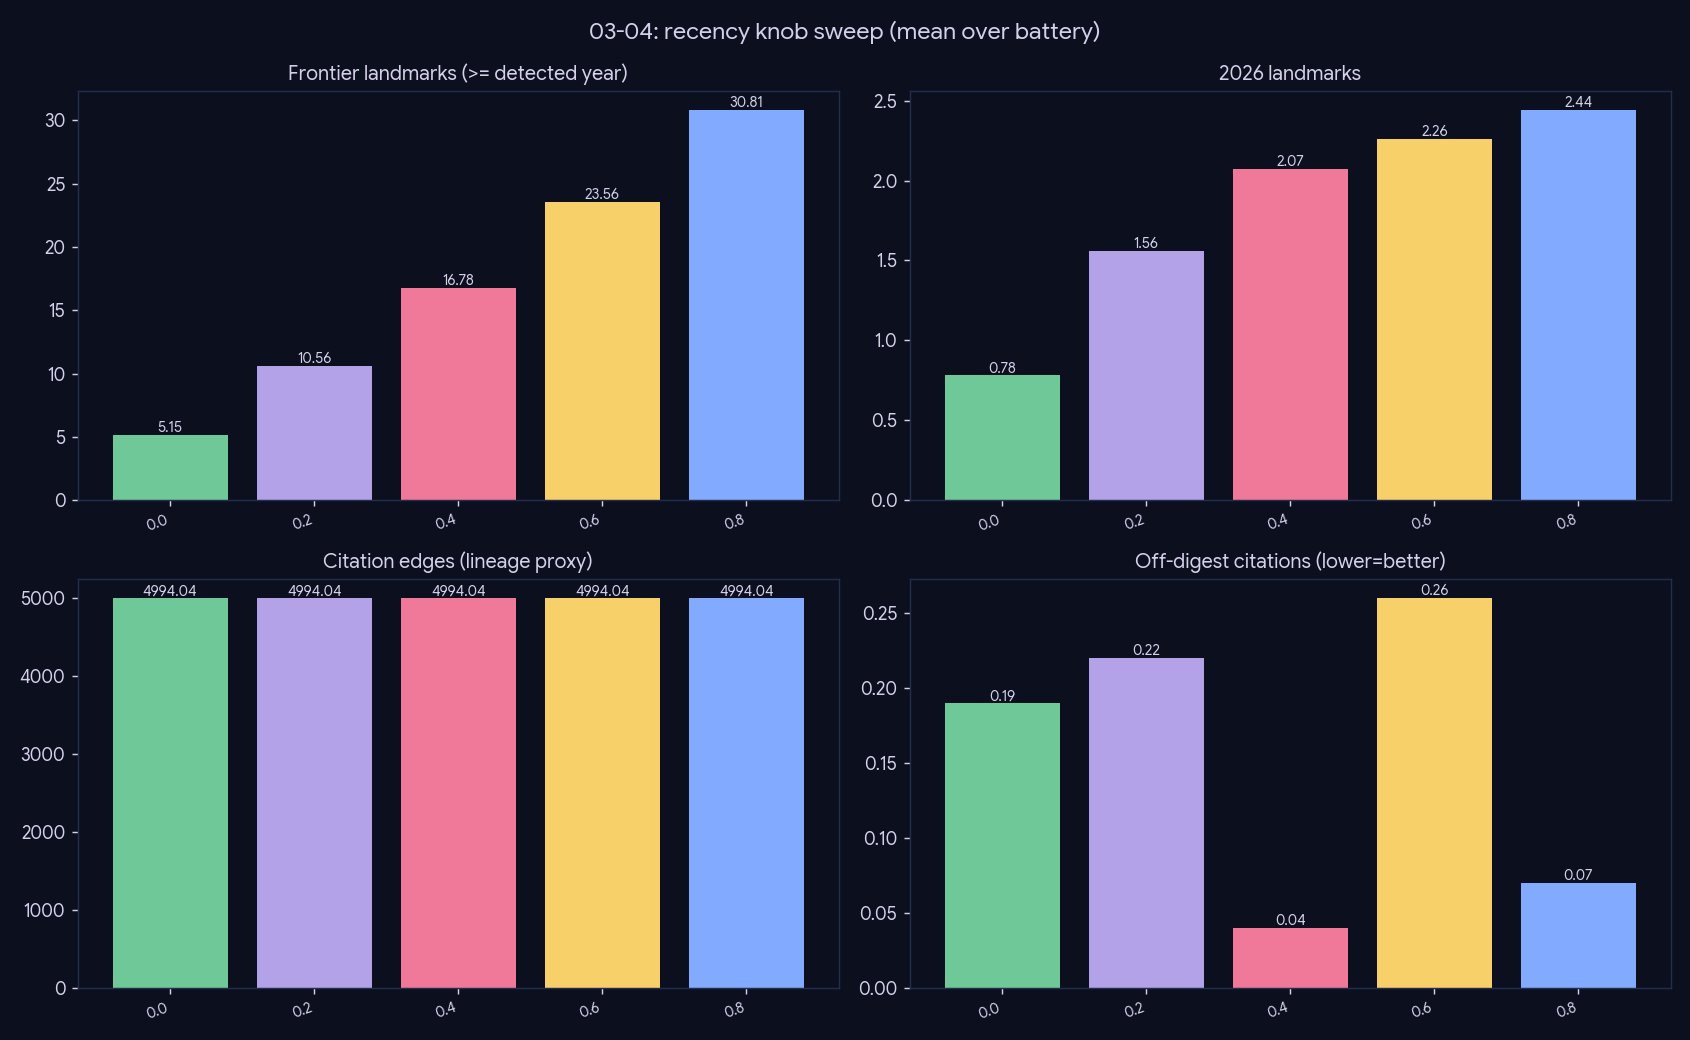
\includegraphics[width=0.95\textwidth]{../results/ablation.png}\end{center}

\section*{Conclusion}
\textbf{Recency is a control surface, not a lever with a single optimum.} Frontier landmarks climb
monotonically with the knob (\rzFrontier{} at $0.0\rightarrow$ \reFrontier{} at $0.8$) while
\texttt{grounded} stays roughly flat ($\sim$22--25) and \texttt{off\_digest} stays low throughout ---
i.e.\ the knob trades \emph{lineage depth for frontier coverage at constant grounding}, exactly as
designed. There is no universal best value: a ``foundations of X'' question wants low recency
(lineage), a ``latest in X'' question wants high. So it is correctly \emph{exposed} as a per-query
knob with a sensible mid default, not tuned to a constant. \textbf{Caveat:} \texttt{landmark\_recall}
is diluted by the non-gold topics and is flat here; the meaningful signal is the monotonic
frontier/lineage trade, which is clean.

\end{document}
